\documentclass[10pt]{article}
\usepackage{icmlko}

\icmlmeta{IP 파운데이션 월드모델}{310}{큰 데서 빌리는 게 아니라 닮은 데서 빌린다}{도서가 누구에게서 빌리는지 재기 전에 순서를 예측해 못 박았다 --- 판에서 제일 큰 도메인이 제일 적게 빌려 준다}

\begin{document}

\twocolumn[
\icmlheader

\begin{abstract}
노트 303이 도서가 제 점수의 3분의 1을 빌린다고 재고 ``\textbf{누구에게서}''를
남겼다. 학습 풀에서 도메인을 하나씩 빼서(leave-one-out) 쟀다. \textbf{재기
전에 순서를 예측해 못 박았다} --- 도서가 빌리는 아홉 축(검색 셋 · 달력 여섯)을
열 도메인 중 여덟이 \textbf{100\% 덮으므로} 덮음은 안 가르고, 가르는 것은
\emph{그 축이 그 도메인에서 ``새롭다''인가}(노트 300의 검사 ③)라고 적었다.
\textbf{결정적 대조는 세계애니}였다 --- 학습 2,648행으로 판에서 제일 큰데
도서가 빌리는 아홉 축 중 ``새롭다''가 \textbf{0개}다. \emph{크기}가 원인이면
제일 크게, \emph{공유된 유익한 구조}가 원인이면 제일 적게 떨어져야 한다.
\textbf{두 설명이 정반대를 예측한다.} 쟀다. \textbf{웹툰 $-$0.0773}
($t{=}{-}2.27$) · 애니 $-$0.0587 · 만화 $-$0.0491 · 모바일 $-$0.0341 ·
시장팝업 $-$0.0222 · 게임 $-$0.0217 · \textbf{세계애니 $-$0.0125} · 아이돌
$-$0.0106. \textbf{예측한 상위 넷이 그대로 나왔고 세계애니는 여덟 중
일곱째다.} 수로도 갈린다 --- 빌린 양과 \textbf{학습행}의 상관이 $+$0.405
($p{=}0.32$)인데 \textbf{``새롭다'' 개수}와는 $+$\textbf{0.803}($p{=}0.016$)
이다. 웹툰은 세계애니보다 학습이 \emph{적은데}(2,106 대 2,648) 빌려 주는 것은
\textbf{6.2배}다. \textbf{파운데이션이 크기로 도는 게 아니라 구조 겹침으로
돈다.}
\end{abstract}
]

\section{재기 전에 순서를 적었다}

노트 303이 도메인마다 빌린 양을 재고 도서 35\%(위키 정정 뒤 32\%) · 펀딩
44\%(43\%)를 냈다. 남은 물음이 ``누구에게서''였다.

\paragraph{방법} 학습 풀에서 도메인을 하나씩 뺀다 --- 그 도메인의 학습 구간
라벨을 결측으로 만든다. 도서의 유보 $\rho$ 가 내려간 만큼이 그 도메인의
몫이다. 축을 끄는 노트 301 · 303과 같은 결의 반사실이다.

\paragraph{두 설명이 있었다}

\begin{center}\small
\begin{tabular}{ll}
\hline
\textbf{크기} & 큰 학습 풀에서 배운 것이 많으니 \\
& 큰 도메인을 빼면 많이 잃는다 \\
\textbf{구조} & 그 축이 \emph{그 도메인에서} 유익해야 \\
& 도서 행에 옮길 것이 생긴다 \\
\hline
\end{tabular}
\end{center}

가르려면 \textbf{크고 구조가 없는} 도메인이 필요하다. 있었다.

\begin{center}\footnotesize
\begin{tabular}{lrr}
\hline
도메인 & 학습행 & 도서의 아홉 축 중 ``새롭다'' \\
\hline
\textbf{세계애니} & \textbf{2,648} & \textbf{0} \\
웹툰 & 2,106 & 6 \\
만화 & 1,783 & 3 \\
모바일 & 1,559 & 3 \\
애니 & 1,467 & 6 \\
펀딩 & 320 & 0 \\
게임 & 259 & 3 \\
시장팝업 & 101 & 0 (덮음 0\%) \\
아이돌 & 54 & 2 \\
\hline
\end{tabular}
\end{center}

\textbf{덮음은 안 가른다} --- 시장팝업만 빼면 여덟이 그 아홉 축을 100\%
덮는다. 예측 순서를 \texttt{preregister\_fromwhom.json} 에 적었다:
\textbf{웹툰 > 애니 > 만화 > 모바일 > 게임 > 아이돌 > 세계애니 > 펀딩}.

\section{구조가 이겼다}

\begin{figure*}[t]
\centering
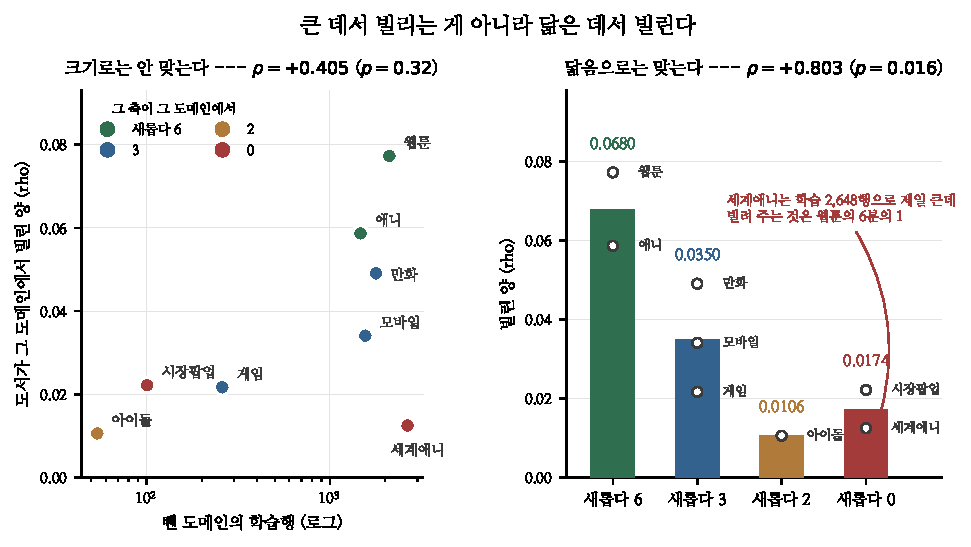
\includegraphics[width=\textwidth]{figs/whom.pdf}
\caption{왼쪽 --- 뺀 도메인의 학습행 대 도서가 빌린 양(색은 그 축이 그
도메인에서 ``새롭다''인 개수). 오른쪽 --- ``새롭다'' 무리별 평균.}
\end{figure*}

\begin{center}\footnotesize
\begin{tabular}{lrrrr}
\hline
뺀 도메인 & 학습행 & 도서 $\rho$ & 빌림 & $t$ \\
\hline
\textbf{웹툰} & 2,106 & 0.3122 & \textbf{0.0773} & $-$2.27 \\
\textbf{애니} & 1,467 & 0.3308 & \textbf{0.0587} & $-$2.03 \\
만화 & 1,783 & 0.3404 & 0.0491 & $-$1.93 \\
모바일 & 1,559 & 0.3554 & 0.0341 & $-$1.65 \\
시장팝업 & 101 & 0.3673 & 0.0222 & $-$1.15 \\
게임 & 259 & 0.3678 & 0.0217 & $-$0.88 \\
\textbf{세계애니} & \textbf{2,648} & 0.3770 & \textbf{0.0125} & $-$0.61 \\
아이돌 & 54 & 0.3789 & 0.0106 & $-$0.39 \\
\hline
\end{tabular}
\end{center}

(기준 도서 $\rho{=}0.3895$. 팝업은 학습 16행이 문턱 아래라 적합에 아예 안
들어가고 짝SE 가 0 이다 --- 잴 것이 없다.)

\paragraph{예측한 상위 넷이 그대로다} 웹툰 > 애니 > 만화 > 모바일. 그리고
\textbf{세계애니가 여덟 중 일곱째}다.

\paragraph{수로도 갈린다}

\begin{center}\small
\begin{tabular}{lrr}
\hline
빌린 양과의 상관 & spearman & $p$ \\
\hline
학습행 & $+$0.405 & 0.32 \\
\textbf{``새롭다'' 개수} & \textbf{$+$0.803} & \textbf{0.016} \\
\hline
학습행 통제 후 ``새롭다'' & $+$0.595 & \\
``새롭다'' 통제 후 학습행 & $+$0.524 & \\
\hline
\end{tabular}
\end{center}

\begin{center}\footnotesize
\begin{tabular}{lrl}
\hline
``새롭다'' & 평균 빌림 & 도메인 \\
\hline
6 & \textbf{0.0680} & 웹툰 · 애니 \\
3 & 0.0350 & 만화 · 모바일 · 게임 \\
2 & 0.0106 & 아이돌 \\
0 & 0.0174 & 시장팝업 · 세계애니 \\
\hline
\end{tabular}
\end{center}

\paragraph{결정적 대조} \textbf{세계애니 2,648행 · ``새롭다'' 0개 $\to$
빌림 0.0125.} \textbf{웹툰 2,106행 --- 더 적은데 --- ``새롭다'' 6개 $\to$
빌림 0.0773.} \textbf{6.2배}다. 크기 설명은 정확히 반대를 예측했다.

\section{그래서 파운데이션이 무엇으로 도는지가 바뀐다}

\begin{center}\footnotesize
\begin{tabular}{ll}
\hline
안 되는 말 & 자료를 더 모으면 전이가 는다 \\
되는 말 & \textbf{그 축이 유익한 도메인}을 모으면 전이가 는다 \\
\hline
\end{tabular}
\end{center}

세계애니는 이 판에서 제일 큰 학습 풀인데 도서에게 거의 아무것도 안 준다.
그 축들이 세계애니에서 라벨과 무관하기 때문이다 --- 세계애니는 달력이
안 통하는 도메인이고(노트 300이 검사 ③ 으로 잰 것) 그러면 \textbf{도서에게
옮겨 줄 달력 구조 자체가 없다.}

\paragraph{그리고 이것이 오래 열린 갈래를 건드린다} ``달력이 왜 트리에서만
되는지''는 설명 넷이 실패하고 관측으로 남아 있다. 이 노트가 다섯째 후보를
준다 --- \textbf{달력은 도메인마다 다르게 작동하고}(웹툰 · 애니에서는
새롭고 세계애니 · 도서에서는 아니다) \textbf{나무만 그 조건부를 표현한다.}
선형은 달력 계수를 하나로 묶으므로 옮길 것이 없다. 아직 안 쟀다 ---
같은 마스크 실험을 F6 · F9 로 돌리면 갈린다.

\paragraph{남은 것}
\begin{center}\small
\begin{tabular}{ll}
\hline
갈래 & 왜 \\
\hline
같은 실험을 선형으로 & 달력 갈래의 다섯째 설명 \\
펀딩도 LOO & 도서와 같은 데서 빌리나 \\
문턱 넘는 게 없다 & 도서 유보 163행 · $|t|$ 최대 2.27 \\
``새롭다''를 지도로 & 누구를 모을지 고른다 \\
\hline
\end{tabular}
\end{center}

\paragraph{규약} \textbf{두 설명이 정반대를 예측하는 자를 찾아라.} 이 판에는
크기와 구조가 대체로 같이 가는 도메인이 많다(웹툰 · 애니는 크고 구조도 있다).
그런 자에서는 아무리 재도 안 갈린다. \textbf{세계애니 하나가 갈랐다} ---
제일 큰데 구조가 0 인 유일한 도메인이다. 그리고 \textbf{순서를 미리 적으니
맞은 것과 틀린 것이 같이 보인다}(상위 넷 적중 · 게임과 아이돌 자리 바뀜).
$|t|$ 가 하나도 2.77 을 못 넘으므로 \textbf{개별 도메인은 못 가른다} ---
갈린 것은 \emph{순서}이고 그것이 이 노트가 주장하는 전부다.

\end{document}
